\section{The image reconstruction problem of radio interferometers}
\begin{figure}[htp]
	% preliminary
	\sbox\twosubbox{%
		\resizebox{\dimexpr.8\textwidth-1em}{!}{%
			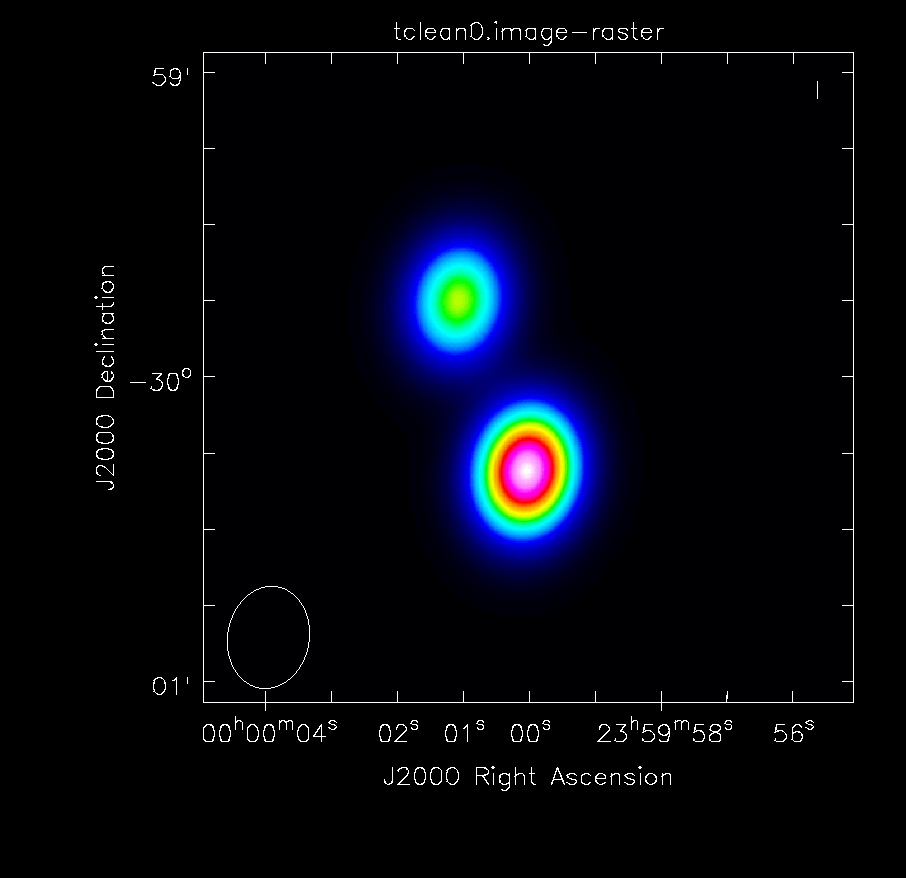
\includegraphics[height=3cm]{./chapters/01.intro/first.png}%
			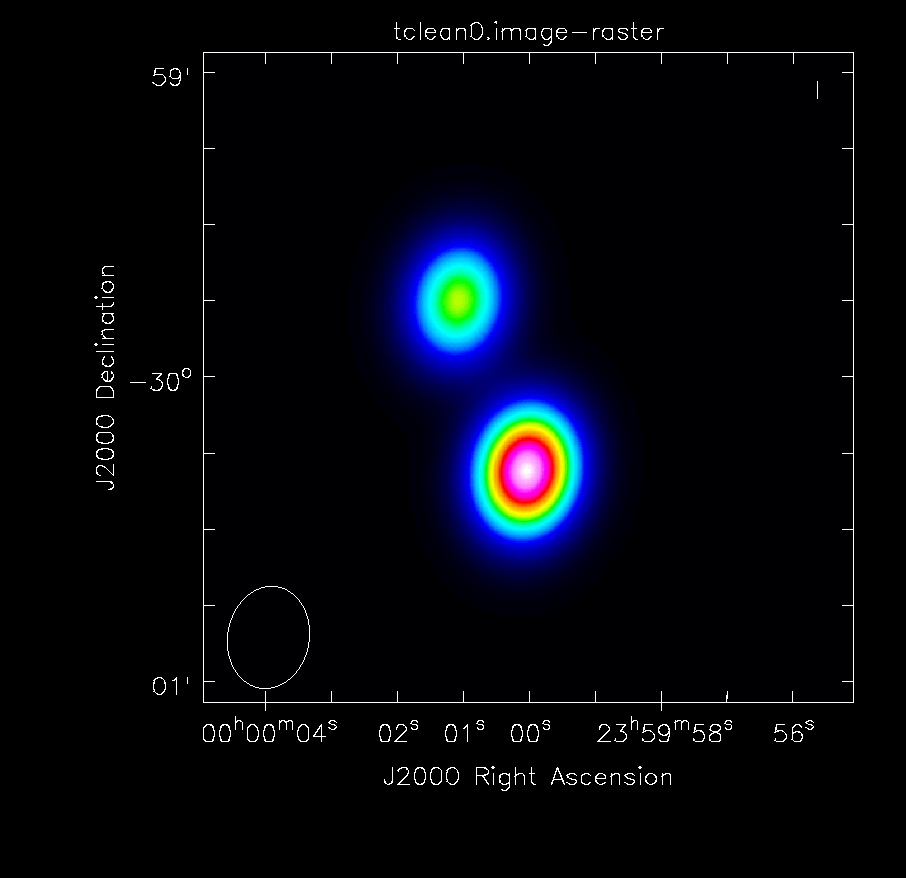
\includegraphics[height=3cm]{./chapters/01.intro/first.png}%
		}%
	}
	\setlength{\twosubht}{\ht\twosubbox}
	
	% typeset
	\centering
	\subcaptionbox{Measurements of the interferometer in the Fourier space.\label{intro0:inversefig:uvspace}}{%
		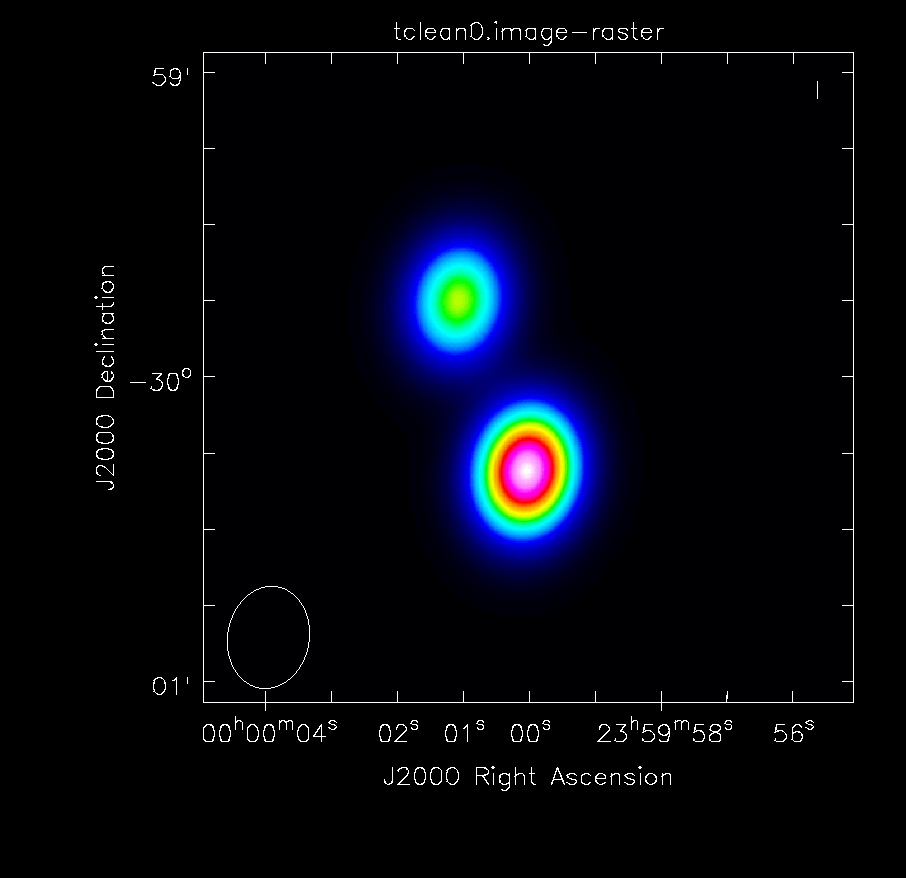
\includegraphics[height=\twosubht]{./chapters/01.intro/first.png}%
	}\quad
	\subcaptionbox{Observed image of the sky, showing two stars.\label{intro0:inversefig:reconstruction}}{%
		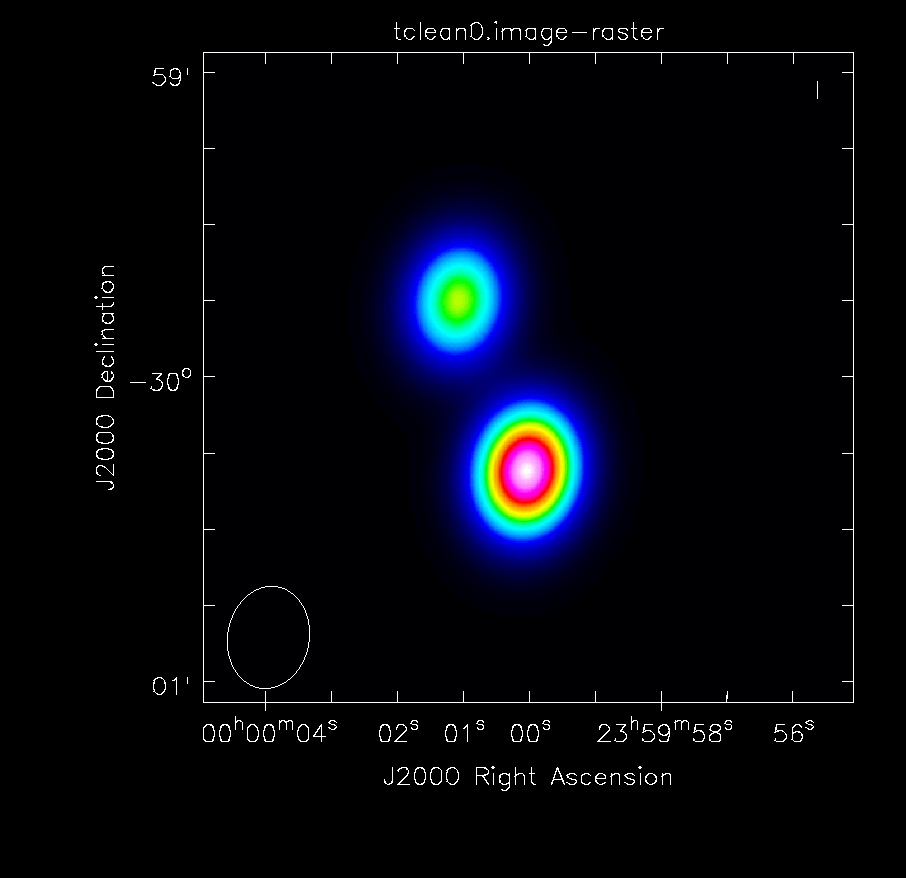
\includegraphics[height=\twosubht]{./chapters/01.intro/first.png}%
	}
	\caption{The image reconstruction problem, the observed image has to be reconstructed from the Fourier measurements.}\label{intro0:inversefig}
\end{figure}

In Radio Astronomy, the angular resolution of a single antenna is limited by the dish-diameter. Of course, there is a practical limit on the size of antenna-dishes we can build. Radio interferometers go around this problem. They use several smaller antennas together, acting like a single large dish. Several smaller dishes together can achieve higher angular resolution than single-dish instruments.

But there are drawbacks. First, the interferometer does not measure the sky in pixels. It measures the amplitude and phase of Fourier components at a given $u$ and $v$ location\footnote{$u$ and $v$ are the axis in Fourier space}. The observed image has to be reconstructed from the measurements. The figure \ref{intro0:inversefig} shows an example of the image reconstruction problem. The figure \ref{intro0:inversefig:uvspace} shows the measurements in the Fourier space, and the figure \ref{intro0:inversefig:reconstruction} shows the observed image of the sky, with two stars close to each other. The image reconstruction has to find the observed image \ref{intro0:inversefig:reconstruction} from the measurements \ref{intro0:inversefig:uvspace}. 

At first glance, we might believe that the image reconstruction is trivial: The interferometer measures Fourier components, and efficient algorithms for the inverse Fourier transforms are well-known. However, two properties of the measured Fourier components make the image reconstruction difficult: The measurements are both noisy and incomplete.

For example the ionosphere of the earth is a source for noise in the measurement. It adds noise to the amplitude and phase of each measured Fourier component. The ionosphere changes over time and can under the right circumstances introduce a high level of noise compared to the signal. The ideal image reconstruction should be able to find the observed image from very noisy Fourier measurements.

The interferometer measures an incomplete set of Fourier components note that the figure \ref{intro0:inversefig:uvspace} does not contain a noisy measurement of every non-zero Fourier component. There are Fourier components with non-zero amplitudes that the interferometer has not seen. The reconstruction algorithm has to find the observed image even though important Fourier components are missing from the measurements.

These two difficulties, the noise and the incomplete measurements make the image reconstruction an ill-posed inverse problem. There are many different images that fit the measurements, and from the measurements alone, we cannot decide which is the truly observed image. 

Numerical optimization algorithm that finds the optimal trade-off between being as close to the data, and being as consistent with our prior knowledge as possible.

Introduce some prior knowledge and return the most-likely observed image given the measurements.

Describe the solution
Reconstruction algorithm


A reconstruction algorithm that can:
\begin{enumerate}
	\item The best possible resolution from the measurements
	\item Is robust to even heavy noise in the measurements.
	\item Uses as few computing resources as possible.
\end{enumerate}

There is no reconstruction algorithm that solves all three problems.

Furthermore a radio interferometers produce an ever increasing volume of Fourier measurements. Recently, the new MeerKAT radio interferometer was completed. It can produce roughly 80 million Fourier components every second, and a single observation may be conducted over several hours. Reconstructing an image for radio interferometers is therefore a big data problem.


We need distributed algorithms.

The CLEAN algorithm, staple in radio astronomy.
Is robust and so far one of the faster algorithms

Big data problem is not sovled. Not every part is of the image reconstruction is distributed


This Project focuses on the third point, distributed image reconstruction with real-world meerkat observations
Received from SARAO for the purpose of algorithmic validation.
